\documentclass[11pt]{preprint}

\usepackage{amsmath, amssymb, amsthm, graphicx, hyperref}

\setlength{\topmargin}{0mm} \setlength{\oddsidemargin}{0mm}
\setlength{\textwidth}{160mm} \setlength{\textheight}{215mm}

\usepackage{amssymb,amsmath,amscd,amsthm}

\title{Discrete Mathematics, Sect 001, 2016 Fall - Quiz 10}
\author{Name:}
\institute{Courant Institute of Mathematical Sciences, NYU}

\newtheorem*{proposition}{Proposition}



\begin{document}

\maketitle

This quiz is scheduled for 15 minutes. No outside notes or calculators are permitted. To get full credit  in all of the problems, use rigorous justification and unless otherwise indicated, make sure that your solution reads as a perfect English sentence. You should only assume the notion of integers, operations, order relations and geometrical objects as given. If you use a statement or a definition from the textbook, make sure to indicate it.
\vspace{0.2cm}


\begin{enumerate}
\item Consider the following graph $G$:

\begin{figure}[h]
\centering
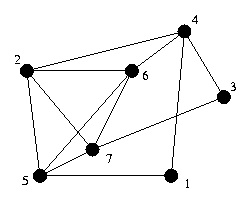
\includegraphics[scale=1]{Euler.jpg}
\end{figure}

\begin{enumerate}
\item (8 Points) Draw the subgraph $G[1,4,5,6]$ induced on the vertex set $\{1,4,5,6\}$.\vspace{3cm}
\item (6 Points) Find the minimum and maximum degree $\delta(G)$ and $\Delta(G)$.\vspace{1cm}
\item (6 Points) Find the clique number $\omega(G)$ and the independence number $\alpha(\bar{G})$\\ (Warning: This is not $\alpha(G)$ being asked).\vspace{3cm}
\end{enumerate}
\end{enumerate}
\end{document}